%!TEX root = main.tex

\section{Decision Procedure for $\strline_{\sf reg}$} \label{sec:decision}

The goal of this section is to prove Theorem~\ref{thm-main}, i.e., the decidability of the path feasibility of $\strline_{\sf reg}$. 
We first show that semantically equivalent PSSTs can be effectively constructed from the $\extract$, $\replace$, and $\replaceall$ functions. 


\begin{lemma}\label{lem-str-fun-to-psst}
For each string function $f = \extract_{i,e}$, $\replace_{\pat, \rep}$, or $\replaceall_{\pat, \rep}$, a PSST $\cT_f$ can be constructed such that 
$\cR_{f} = \{(w, w') \mid w'= f(w)\}.$
\end{lemma}



%\begin{lemma}\label{lem-replace}
%A PSST $\cT_{\replace_{\pat, \rep}}$ (resp. $\cT_{\replaceall_{\pat, \rep}}$) can be constructed for $\replace_{\pat, \rep}$ (resp. $\replaceall_{\pat, \rep}$) such that $\cR_{\cT_{\replaceall_{\pat, \rep}}} = \{(w, w') \mid w'= \replaceall_{\pat, \rep}(w)\}$ (resp. $\cR_{\cT_{\replaceall_{\pat, \rep}}} = \{(w, w') \mid w'= \replaceall_{\pat, \rep}(w)\}$).
%\end{lemma}
%
The proof is given in Appendix~\ref{appendix:sec-extract-replace-to-psst}.
With Lemma~\ref{lem-str-fun-to-psst}, the path feasibility of $\strline_{\sf reg}$ reduces to path feasibility of string-manipulating programs consisting of  a sequence of the statements of the form $z:=x \concat y$, $y:=\cT(x)$, and $\ASSERT{x \in \cA}$, where $\cT$ is a PSST and $\cA$ is an FA.  The class of programs is denoted by $\strline'_{\sf reg}$. We then  follow %the %backward computation %reasoning approach of 
the backward reasoning approach proposed in \cite{CCH+18,CHL+19} to solve the path feasibility of $\strline'_{\sf reg}$, where the key is to show that the pre-images of regular languages  under PSSTs  are regular and can be computed effectively.


\begin{definition}[Pre-image]
For a string relation $R \subseteq \Sigma^* \times (\Sigma^* \cup \{\nullchar\})$ and $L \subseteq \Sigma^*$, we define the \emph{pre-image} of $L$ under $R$ as $R^{-1}(L):=\{w \in \Sigma^* \mid \exists w'.\ w' \in L \mbox{ and } (w, w') \in R\}$. 
\end{definition}


 \begin{lemma}[Pre-image of regular languages under PSSTs]
  \label{lem:psst_preimage}
  Given a PSST $\psst = (Q_T, \Sigma$, $X$, $\delta_T$, $\tau_T$, $E_T$,  $q_{0, T}$, $F_T$) and an \FA{} $\Aut
  = (Q_A, \Sigma, \delta_A, q_{0, A}, F_A)$, we can compute an \FA{} $\cB = (Q_B,
  \Sigma, \delta_B, q_{0, B}, F_B)$ in exponential time  such that $\Lang(\cB) = \cR^{-1}_{\cT}(\Lang(\Aut))$.
\end{lemma}

The proof of Lemma~\ref{lem:psst_preimage} is given in Appendix~\ref{app-pre-image}.
With Lemma~\ref{lem:psst_preimage}, we  solve the path feasibility of $\strline'_{\sf reg}$ by repeating the following procedure, until no more assignment statements are left. Let $S$ be the current $\strline'_{\sf reg}$ program.
\begin{itemize}
\item If the last assignment statement of $S$ is $y:=\cT(x)$, then let $\ASSERT{y \in \cA_1}$, $\cdots$, $\ASSERT{y \in \cA_n}$ be an enumeration of all the assertion statements for $y$ in $S$. Compute $\cR^{-1}_\cT(\Lang(\cA_1))$ as an FA $\cB_1$, $\cdots$, and $\cR^{-1}_\cT(\Lang(\cA_n))$ as $\cB_n$. Remove  the assignment  $y:=\cT(x)$ and add the assertion statements $\ASSERT{x \in \cB_1}$; $\cdots$; $\ASSERT{x \in \cB_n}$. 
%
\item If the last assignment statement of $S$ is $z:=x \concat y$, then let $\ASSERT{z \in \cA_1}$, $\cdots$, $\ASSERT{z \in \cA_n}$ be an enumeration of all the assertion statements for $z$ in $S$. Compute $\concat^{-1}(\Lang(\cA_1))$, the pre-image of $\concat$ under $\Lang(\cA_1)$, as a collection of FA pairs $(\cB_{1,j}, \cC_{1,j})_{j \in [m_1]}$, $\cdots$, and $\concat^{-1}(\Lang(\cA_n))$ as $(\cB_{n, j}, \cC_{n,j})_{j \in [m_n]}$ (c.f. \cite{CHL+19}). Remove the assignment $z:=x \concat y$, nondeterministically choose the indices $j_1 \in [m_1], \cdots, j_n \in [m_n]$, and add the assertion statements $\ASSERT{x \in \cB_{1,j_1}}; \ASSERT{y \in \cC_{1, j_1}}$; $\cdots$; $\ASSERT{x \in \cB_{n,j_n}}; \ASSERT{y \in \cC_{n, j_n}}$. 
\end{itemize}
Let $S'$ be the resulting $\strline'_{\sf reg}$ program containing no assignment statements. Then the path feasibility of $S'$ can be solved by checking the nonemptiness of the intersection of regular constraints for the input variables, which is known to be \pspace-complete \cite{Kozen77}.


\paragraph*{Complexity analysis.} Because the pre-image computation for each PSST incurs an exponential blow-up, the aforementioned decision procedure has a non-elementary complexity in the worst-case. Nevertheless, since the number of PSSTs is usually small in the path constraints of string-manipulating programs, the performance of the decision procedure is actually good on the benchmarks we tested, with the average running time per query a few seconds (see Section~\ref{sect:impl}).



\begin{remark}
The procedure above extends the backward-reasoning approach in \cite{CHL+19}, since standard one-way and two-way finite-state transducers were considered therein and PSSTs, in particular priorities, are beyond them\footnote{It is known that deterministic streaming string transducers are expressively equivalent to two-way deterministic finite-state transducers, which, nevertheless, is not the case for nondeterministic transducers \cite{AC10,AD11}.}. 
%, PSSTs we introduce PSST, a new transducer model that covers the $\extract_{i,e}$ and $\replaceall_{\sf pat, rep}$ functions, where priorities are used to model the greedy/non-greedy semantics of $*$/$*?$ and string variables are used to store the matches of capturing groups. 
\end{remark}

%It remains to prove Lemma~\ref{lem-extract}-\ref{lem:psst_preimage}, which will be the focus of the next two subsections.
% in Section~\ref{sec-extract-replace-to-psst}-\ref{sec-pre-image}.



%%%%%%%%%%%%%%%%%%%%%%%%%%%%%%%%%%%%%%%%%%%%%%%
%\subsection{From $\extract$ and $\replaceall$ to PSST}\label{sec-extract-replace-to-psst}
%
%At first, we can adapt the pNFA construction in \cite{BDM14}, which in turn is a variant of the standard Thompson construction \cite{Thompson68}, and show the following result. 
%
%\begin{proposition}\label{prop-rwre-to-pfa}
%For each $\cgexp$ $e$, a PFA $\cA_e$ can be constructed in linear time such that 
%\begin{itemize}
%\item $\cA_e$ has a unique initial state without incoming transitions and a unique final state without outgoing transitions,
%%
%\item for subexpression $e'$ of $e$, $\cA_e$ contains an isomorphic copy of $\cA_{e'}$ (i.e. the PFA constructed for $e'$), denoted by ${\sf Sub}_{e'}[\cA_e]$. 
%\end{itemize}
%\end{proposition}
%%Let us use ${\sf Sub}_{e'}[\cA_e]$ to denote the isomorphic copy of $\cA_{e'}$ in $\cA_e$, as mentioned in Proposition~\ref{prop-rwre-to-pfa}.
%
%%
%%\begin{theorem}\label{thm-main}
%%The path feasibility of $\strline_{\sf reg}$ is decidable.
%%\end{theorem}
%%
%
%
%
%
%%\subsection{From $\regexp[\sf CG]$ to PFA}
%%\label{construction:pnfa}
%
%%\begin{figure*}
%%	\centering
%%	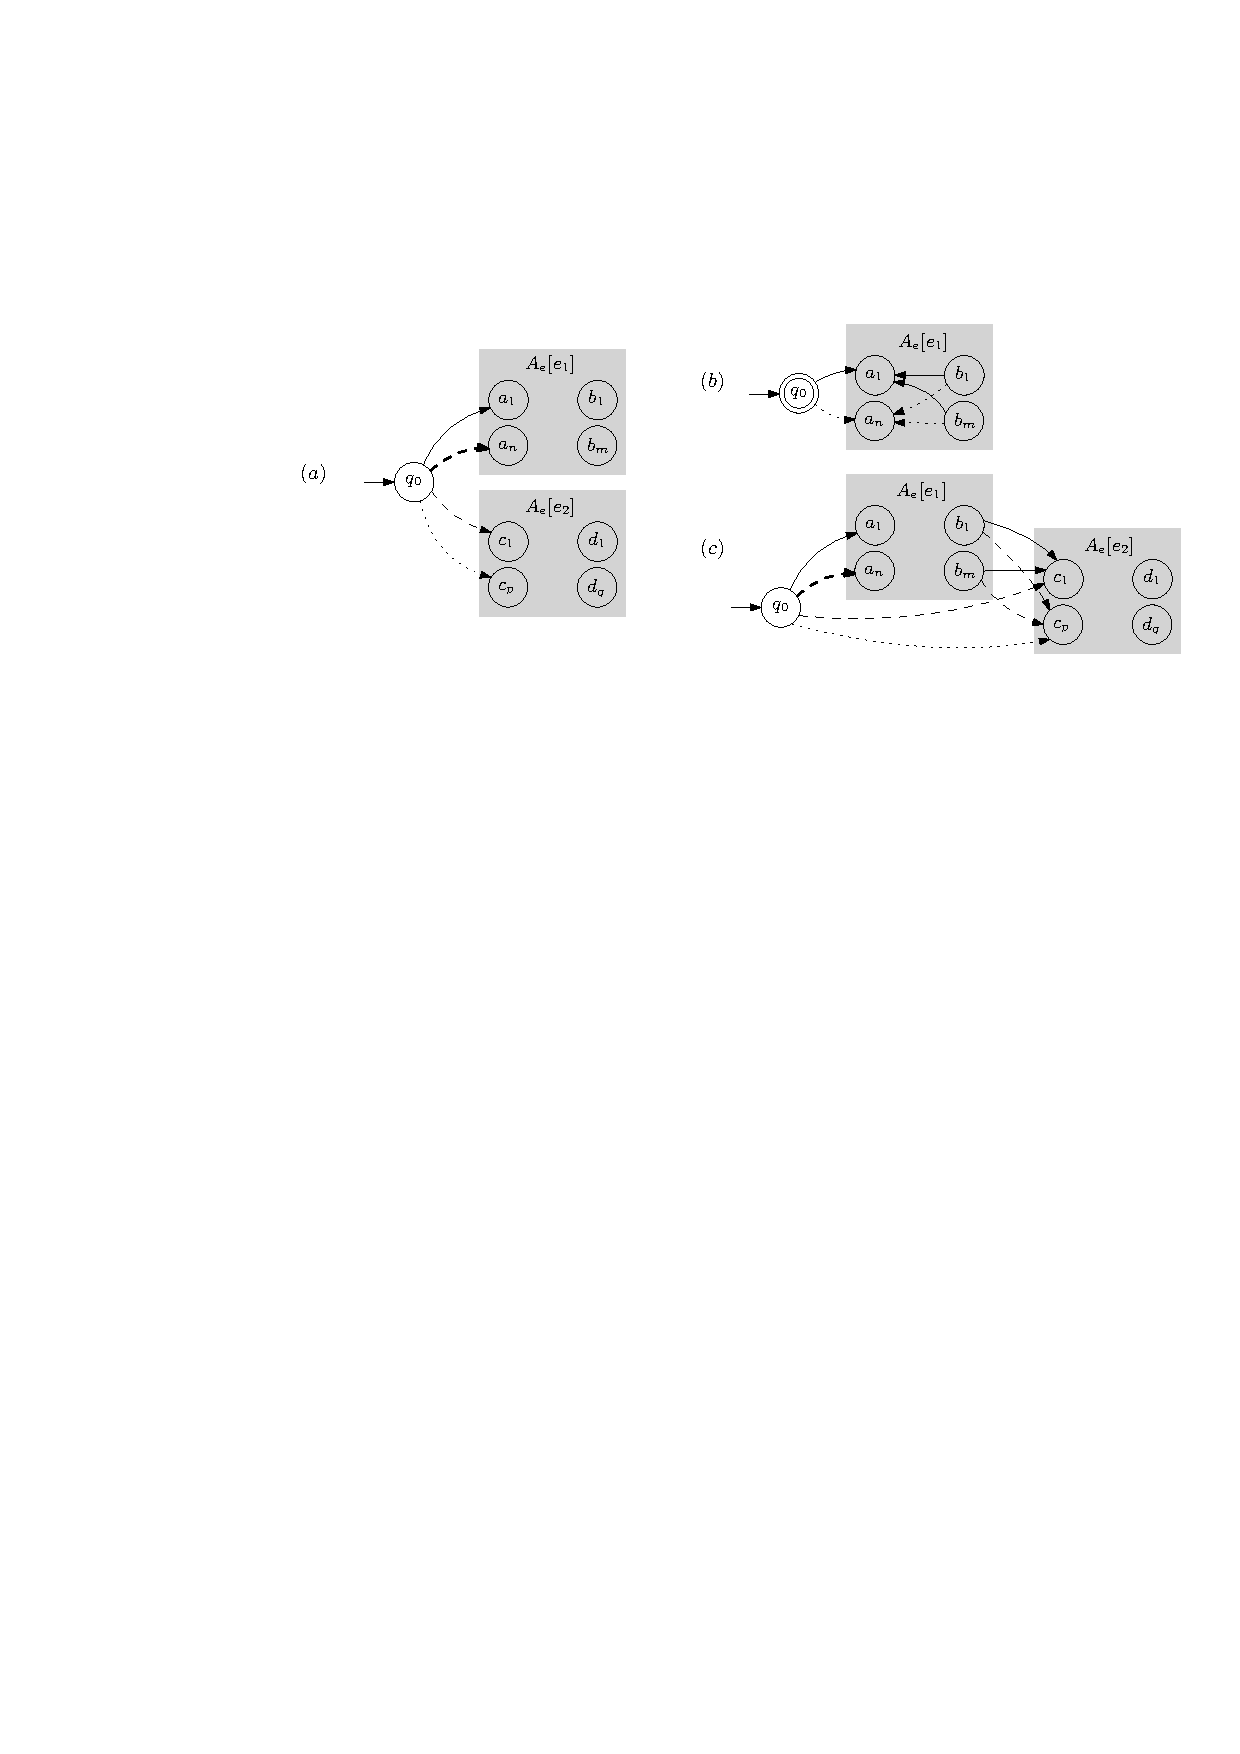
\includegraphics{pglushkov_01}
%%	\caption{pNFA $A_e$ for (a) $e=e_1+e_2$ (b) $e=e_1^{\ast}$ and (c) $e=e_1 \concat e_2$ where $\varepsilon \in \Lang(e_1)$ and $\varepsilon \notin \Lang(e_2)$. A transition of lower priority is depicted thiner and more densely dotted. }
%%	\label{fig:pglushkov}
%%\end{figure*}
%
%%For instance, if $e = (a (ab)^*)^*$ and $e' = a(ab)^*$, then $A_{e}[e']$ is the subgraph of $A_{e}$ comprising the states $\{a_1, a_2, b_3\}$ and the transitions $\{(a_1, a, a_2), (a_2, b, b_3), (b_3, a, a_2)\}$.
% 
%%Figure.\ref{fig:pglushkov} also illustrates the subgraphs corresponding to direct subexpressions of $e$.
%
%
%%\begin{definition}
%%Let $e \in \regexp[\sf CG]$ and $e'$ be a subexpression of $e$. Then a copy of $\cA_{e'}$ in $\cA_e = (Q, \Sigma, \delta, \tau, q_0, f_0)$ is a PFA $(Q', \Sigma, \delta', \tau', q'_0, f'_0)$ such that  
%%\begin{itemize}
%%\item $Q' \subseteq Q$, $q'_0, f'_0 \in Q'$, 
%%\item $\delta'$ is the restriction of $\delta$ to $Q'$, with the outgoing transitions of $f'_0$ removed, specifically, for every $\sigma \in \Sigma$ and $q \in Q' \setminus \{f'_0\}$, $\delta'(q, \sigma) = \delta(q, \sigma)$, $\tau'(q) = \tau(q)$, $\delta'(f'_0, \sigma) = ()$, and $\tau'(f'_0) = ((); ())$,
%%\item $(Q', \Sigma, \delta', \tau', q'_0, f'_0)$ is isomorphic to $\cA_{e'}$.
%%\end{itemize}
%%\end{definition}
%
%%From the aforementioned recursive construction of $\cA_e$, we know that for each subexpression $e'$ of $e$, a PFA for $e'$, which is isomorphic to $\cA_{e'}$, is also constructed. Let us use ${\sf Sub}_{e'}[\cA_e]$ to denote this PFA for $e'$, which, roughly speaking, is a subgraph of $\cA_e$.
%
%
%We are ready to prove Lemma~\ref{lem-extract} and Lemma~\ref{lem-replace}.
% 
%\begin{proof}[Lemma~\ref{lem-extract}]
%%\paragraph*{Construction of $\cT_{\extract_{i,e}}$.} 
%Let $e'$ be the subexpression corresponding to the $i$-th capturing group of $e$. In particular, if $i=0$, then $e' = e$. 
%Suppose $\cA_e = (Q, \Sigma, \delta, \tau, q_0, f_0)$. 
%%Moreover, let $\cA^\dag_e = (Q^\dag, \Sigma, \delta^\dag, \tau^\dag, q^\dag_0, f^\dag_0)$ be an isomorphic copy of $\cA_e$, where every state $q$ in $\cA_e$ is replaced by $q^\dag$ in $\cA^\dag_e$. Let us use ${\sf Sub}_{e'}[\cA^\dag_e]$ to denote the isomorphic copy of ${\sf Sub}_{e'}[\cA_e]$ in $\cA^\dag_e$.
%
%Intuitively, $\cT_{\extract_{i,e}}$ uses a string variable $x$ to store the value of the $i$th capturing group. Initially it assigns $\nullchar$ to $x$ to denote the fact that the capturing group is not matched yet. It then simulates $\cA_e$, and stores letters into $x$ when applying the transitions in ${\sf Sub}_{e'}[\cA_e]$. Finally, it outputs the value of $x$ when $\cA_e$ accepts.
%
%Formally, $\cT_{\extract_{i,e}} = (Q \cup \{q'_0\}, \Sigma, X, \delta', \tau', E', q'_0, F')$ (see Figure~\ref{fig-psst-extract}), where 
%\begin{itemize}
%\item $q'_0 \not \in Q$,
%%
%\item $X = \{x\}$,
%%
%%\item $\delta'$ is obtained from $\delta$ by adding $x: = x\sigma$ for each transition $(q, \sigma, q')$ in ${\sf Sub}_{e'}[\cA_e]$,  
%%
%\item $F'(f_0)= x$ and $F'(p)$ is undefined for all the other states $p \in Q  \cup \{q'_0\}$,
%%
%\item $\delta'$ and $\tau'$ are defined as follows,
%\begin{itemize}
%\item $\tau'(q'_0) = ((q_0); ())$,
%%
%\item $\delta'$ includes all the transitions in $\delta$,
%%
%\item $\tau'$ includes all the transitions in $\tau$,
%%
%\end{itemize}
%%
%\item $E'$ is defined as follows,
%\begin{itemize}
%\item if $q_0$ does not occur in ${\sf Sub}_{e'}[\cA_e]$, then $E'((q'_0, \varepsilon, q_0))(x) = \nullchar$, otherwise, $E'((q'_0, \varepsilon, q_0))(x) = \varepsilon$,
%%
%\item for each transition $(q, \sigma, q')$ in ${\sf Sub}_{e'}[\cA_e]$, $E'((q, \sigma, q'))(x) = x \sigma$,
%% 
%\item for each transition $(q, \sigma, q')$ such that $q$ does not occur not in ${\sf Sub}_{e'}[\cA_e]$ and $q'$ occurs in ${\sf Sub}_{e'}[\cA_e]$, $E'((q, \sigma, q'))(x) = \varepsilon$,
%%
%\item for all the other transitions $t$ of $\cA_e$, $E'(t)(x) = x$.
%\end{itemize}
%%
%%
%\end{itemize}
%
%\begin{figure}[ht]
%\centering
%%\rule{\linewidth}{0cm}
%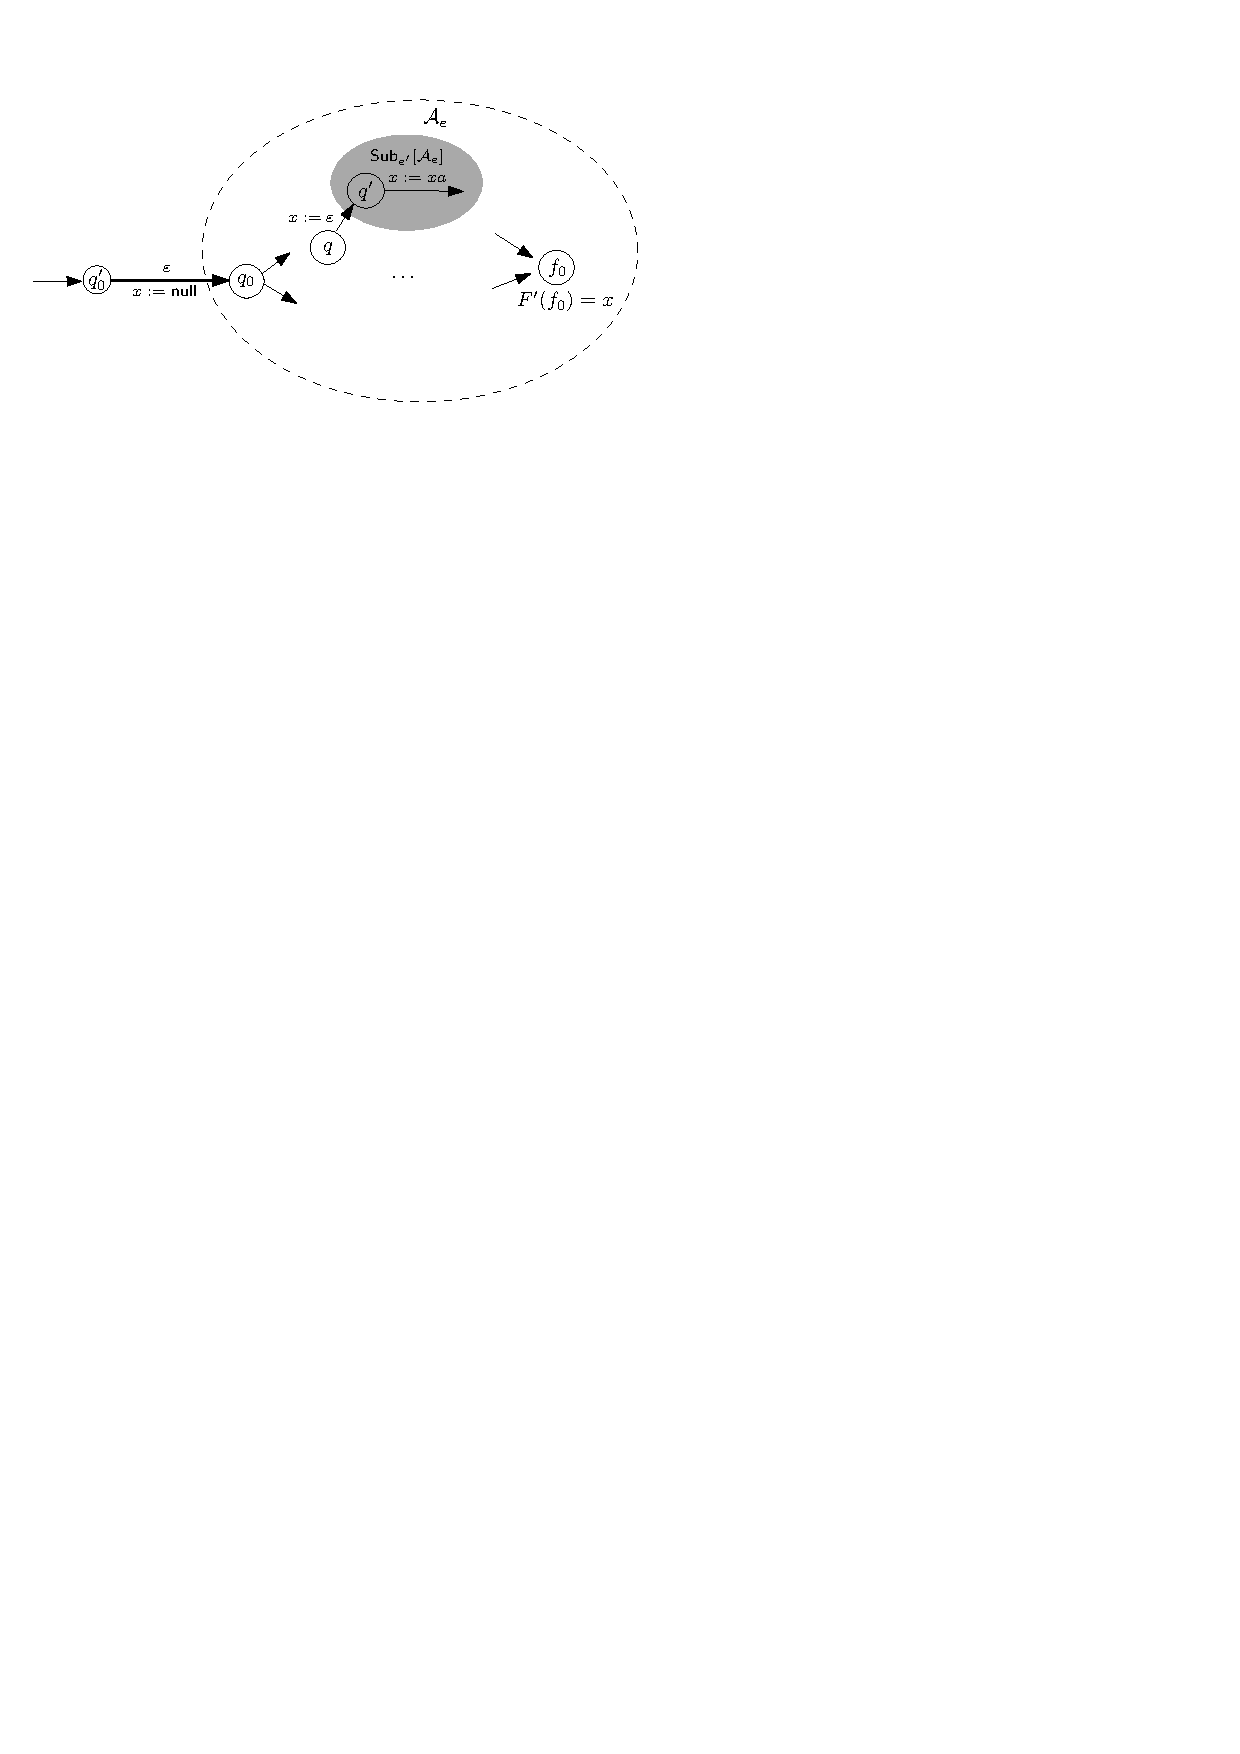
\includegraphics[width = 0.6\textwidth]{psst-extract.pdf}
%\caption{The PSST for $\extract_{i,e}$}
%\label{fig-psst-extract}
%\end{figure}
%\qed
%\end{proof}
%
%
%\begin{proof}[Lemma~\ref{lem-replace}]
%%\paragraph*{Construction of $\cT_{\replaceall_{\pat, \rep}}$.} 
%Let $\$i_1, \cdots, \$i_k$ with $i_1 < \cdots < i_k$ be an enumeration of all the references in $\rep$. 
%Moreover, for every $j \in [k]$, let $e'_{i_j}$ be the subexpression of $\pat$ corresponding to the $i_j$-th capturing group.
%
%Suppose $\cA_\pat = (Q, \Sigma, \delta, \tau, q_0, f_0)$. Then $\cT_{\replace_{\pat,\rep}}$ is obtained from $\cA_\pat$ by adding a fresh states $q'_0$ such that (see Figure~\ref{fig-psst-replace})
%\begin{itemize}
%\item $\cT_{\replace_{\pat,\rep}}$ goes from $q'_0$ to $q_0$ via an $\varepsilon$-transition of higher priority than the non-$\varepsilon$-transitions, in order to search the first match of $\pat$ starting from the current position, 
%%
%\item when $\cT_{\replace_{\pat,\rep}}$ stays at $q'_0$, it keeps appending the current letter to the end of $x_0$, 
%%
%\item starting from $q_0$, $\cT_{\replace_{\pat,\rep}}$ simulates $\cA_\pat$ and stores the matches of the $\$i_1$-th, $\ldots$, $\$i_k$-th capturing groups of $\pat$ into the string variables $x_1, \cdots, x_k$ respectively,   
%%
%\item when the first match of $\pat$ is found, $\cT_{\replace_{\pat,\rep}}$ goes from $f_0$ to $q'_0$ via an $\varepsilon$-transition, appends the replacement string, which is $\rep[x_1/\$_{i_1}, \cdots, x_k/\$_{i_k}]$, to the end of $x_0$, and keeps searching for the next match of $\pat$.
%\end{itemize}
%
%\begin{figure}[ht]
%\centering
%%\rule{\linewidth}{0cm}
%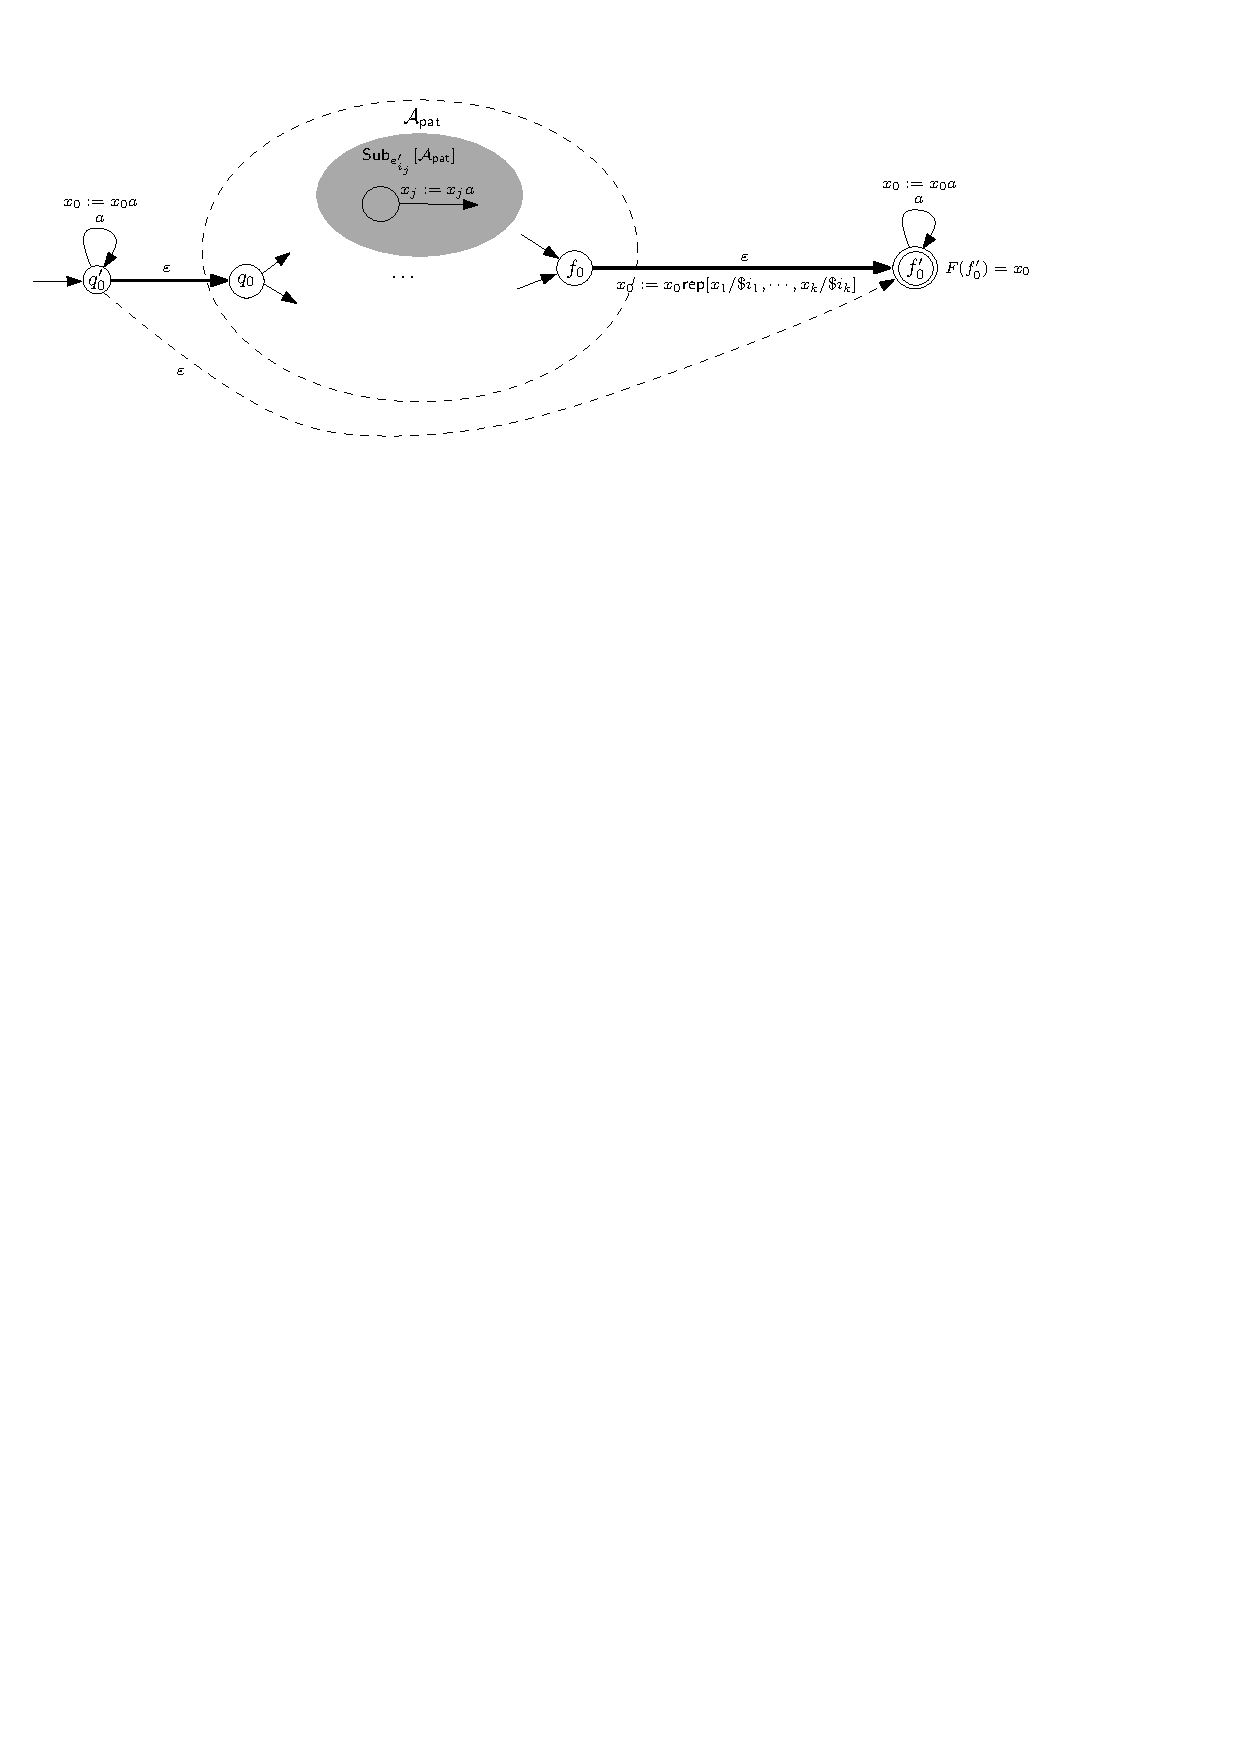
\includegraphics[scale=0.8]{psst-replace.pdf}
%\caption{The PSST for $\replace_{\pat,\rep}$}
%\label{fig-psst-replace}
%\end{figure}
%
%Formally, $\cT_{\replaceall_{\pat, \rep}} =$ $(Q \cup \{q'_0\}$, $\Sigma$, $X$, $\delta'$, $\tau', E, q'_0, F)$ where
%\begin{itemize}
%\item $q'_0 \not \in Q$,
%
%\item  $X = \{x_0, x_1, \cdots, x_k\}$,
%%
%\item $F(q'_0) = x_0$, and $F(q')$ is undefined for every $q' \in Q$,
%%
%\item $\delta'$ and $\tau'$ are obtained from $\delta$ and $\tau$ as follows,
%\begin{itemize}
%\item $\delta'(q'_0, \sigma) = (q'_0)$ for every $\sigma \in \Sigma$, and $\tau'(q'_0) = ((q_0); ())$,
%%
%\item for every $q \in Q \setminus \{f_0\}$ and $\sigma \in \Sigma$, $\delta'(q, \sigma) = \delta(q, \sigma)$ and $\tau'(q) = \tau(q)$, 
%%
%\item $\delta'(f_0, \sigma) = ()$ for every $\sigma \in \Sigma$ and $\tau'(f_0) = ((q'_0); ())$,
%\end{itemize}
%%
%\item $E$ is defined as follows, 
%\begin{itemize}
%\item for every transition $(q, \sigma, q')$ with $\sigma \in \Sigma^\varepsilon$ in $\cA_\pat$, $E(q, \sigma, q')(x_0) = x_0$,
%%
%\item for every transition $(q, \sigma, q')$ with $\sigma \in \Sigma^\varepsilon$ and $j \in [k]$,  if $(q, \sigma, q')$ occurs in ${\sf Sub}_{e'_{i_j}}[\cA_\pat]$, then $E(q, \sigma, q')(x_j) = x_j\sigma$, otherwise, $E(q, \sigma, q')(x_j) = x_j$,
%%
%%\item for all the other transitions $(q, \sigma, q')$ with $\sigma \in \Sigma^\varepsilon$ in $\cA_e$, we have $E(q, \sigma, q')(x) = x$, 
%%
%\item  for every $\sigma \in \Sigma$ and $j \in [k]$, $E(q'_0, \sigma, q'_0)(x_0) = x_0\sigma$ and $E(q'_0, \sigma, q'_0)$$(x_j) = x_j$, 
%
%\item $E(q'_0, \varepsilon, q_0)(x_j) = x_j$ for every $j \in [k] \cup \{0\}$, 
%%
%\item $E(f_0, \varepsilon, q'_0)(x_0) = x_0 \rep[x_1/\$i_1,\ldots, x_k/\$i_k]$, and for every $j \in [k]$, we have $E(f_0, \varepsilon, q'_0)(x_j) = \varepsilon$.
%
%\end{itemize}
%%
%\end{itemize}
%\qed
%\end{proof}

%In the rest of this section, we are going to illustrate how to prove Lemma~\ref{lem:psst_preimage}, namely, how to compute the pre-images of regular languages under PSSTs.

%\subsection{Computing the pre-image of regular languages under PSSTs}\label{sec-pre-image}

%In this subsection, we are going to show Lemma~\ref{lem:psst_preimage}, namely, how to compute the pre-images of regular languages under PSSTs.

%\tl{another way is to first define B as a PFA, could make the construction a bit modular?}\zhilin{Add a counter example for this natural idea.}
 
